\section{Aufbau}

\subsection{Architektur}
Wie bereits im Pflichtenheft angeführt, haben wir uns für eine klare Trennung von Client und Server entscheiden um somit eine höchstmögliche Modularität zu gewährleisten. So können Client- und Server-Anwendung auf getrennten Servern laufen. Die Kommunikation erfolgt über REST-Schnittstellen, was auch in Zukunft die Entwicklung einer App ermöglicht, ohne die Server-Anwendung anpassen zu müssen. \\
Im Folgenden werden die Architekturen von Server und Client näher beschrieben.
\begin{figure}[h]
	\centering
	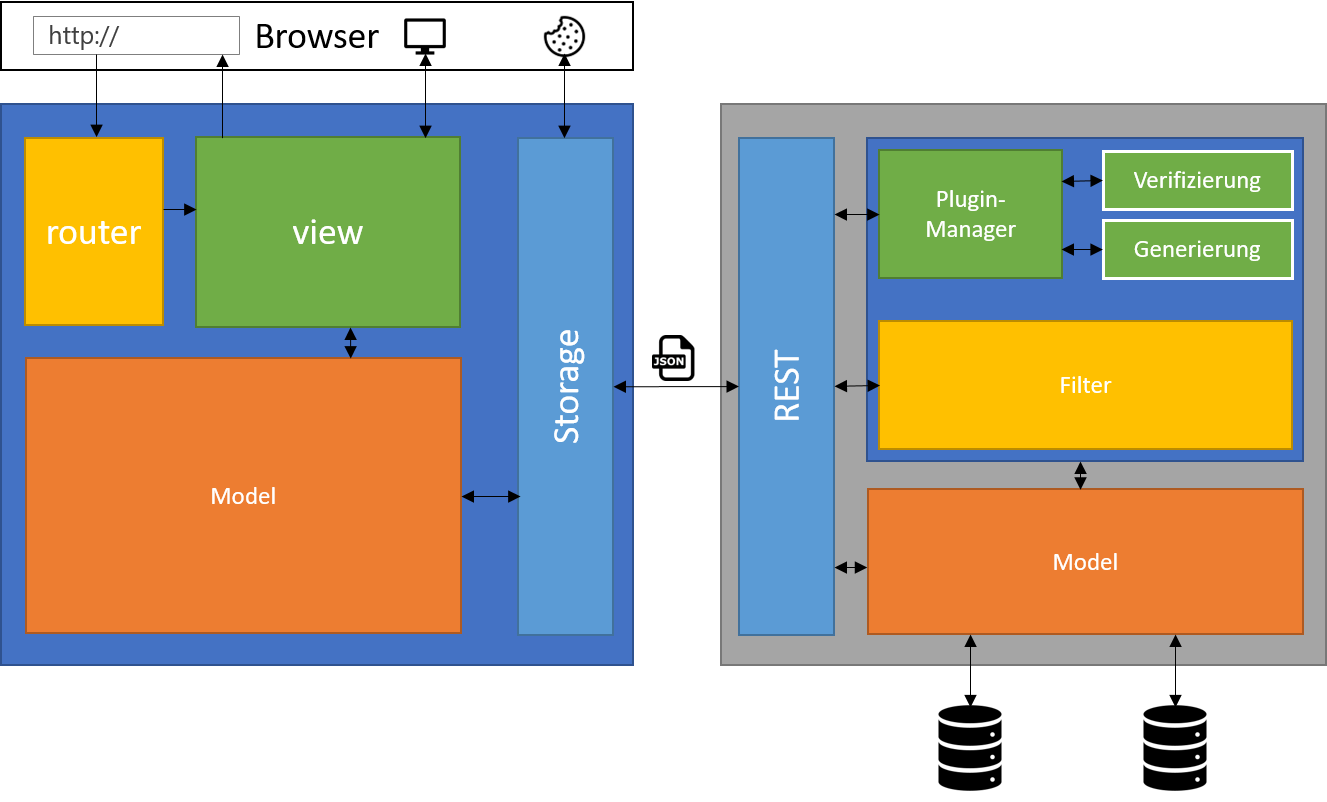
\includegraphics[width=.7\textwidth, clip, trim= {0cm 3cm 0cm 0cm}]{content/diagrams/architecture}
	\caption{Systemarchitektur}
\end{figure}
\subsubsection{Server}
Der Server besteht aus zwei zentralen Komponenten: Dem Paket \texttt{rest}, sowie dem Paket \texttt{model}. \\
Das Paket \texttt{rest} beinhaltet die Schnittstellen zur Außenwelt, denn hier sind alle vorhandenen REST-Webservices der Server-Anwendung in Form von Ressourcen-Klassen mit entsprechenden Methoden implementiert. Des Weiteren beinhaltet das Paket Komponenten zur Erzeugung von JSON-Objekten, sowie zur Zugriffssteuerung auf die Webservices. Im Unterpaket \texttt{authorization.endpoint} befindet sich eine rudimentäre Implementierung eines Identity Providers, der bei Bedarf durch eine andere Implementierung ersetzt werden kann.\\
Das Paket \texttt{model} hingegen stellt die Schnittstelle zum Persistence-Layer bereit. Es enthält zum Einen Modellklassen, welche Datenbankeinträge objektorientiert abbilden. Diese Modellklassen sind in Form einfacher Java-Objekte entworfen, welche nur über Getter und Setter für ihre Attribute verfügen (sog. \emph{POJOs}, Plain Old Java Object). Die Modellklassen sind in Pakete zur Modellierung von Modulen, sowie zur Modellierung von Nutzerdaten und Studienplänen aufgeteilt. Zum Anderen verfügt jedes dieser Modellierungspakete über ein Unterpaket zum eigentlichen Datenbankzugriff über sog. \emph{Data-Access-Objects} (DAO), welche Methoden zum Lesen und Schreiben der Datenbank bereitstellen. Diese sind in Form von Schnittstellen ausgelegt. Die konkrete Implementierung dieser verwendet \emph{JBoss Hibernate} für den Datenbankzugriff, jedoch kann sie jederzeit durch eine andere Datenbankschnittstelle ersetzt werden.\\
Das Paket \texttt{filter} enthält eine Kompositium-basierte Modellierung von Modulfiltern, welche im Zusammenspiel mit den DAOs den selektiven Zugriff auf Module ermöglichen. \\
Das Paket \texttt{pluginmanager} verwendet die \emph{Java ServiceLoader API} um dynamisch Generierungs"= und Verifizierungstools zu laden. Hierfür müssen diese in Form von Jar-Dateien dem Klassenpfad hinzugefügt werden, wodurch ein Austausch von Tools ohne Änderungen an der Anwendung möglich ist. \\
Die Pakete \texttt{generation} und \texttt{verification} enthalten die zu implementierenden Schnittstellen für neue Service Provider, sowie einfache Implementierungen eines Studienplan"=Generators und -Verifizierers. Das Paket \texttt{generation} enthält darüber hinaus noch eine API zur Modellierung von Zielfunktionen, welche von Generatoren verwendet werden können.

\subsubsection{Client}
Der Client besteht aus einer leicht abgewandelten Model"=View"=Controller-Architektur (MVC"=Architektur), die auf Backbone.js \cite{backbone} basiert.
Das System besteht aus 4 Haupt-Paketen: Storage, Model, View und Router.\\
Storage übernimmt die Kommunikation mit dem REST-Webservice sowie die Speicherung in Cookies. Somit bildet Storage die Zugriffsschicht für das Model-Paket. \\
Model bildet die Daten aus den Cookies und dem REST-Webservice auf Klassen ab und stellt Möglichkeiten zum Abruf sowie zur Speicherung zur Verfügung, die auf Storage basieren.\\
View zeigt die Daten aus dem Model an und aktualisiert im Fall einer Änderung des Models die Anzeige. Auch fängt das View-Paket Interaktionen mit der Benutzeroberfläche (wie Klicks oder Drag and Drop) ab und verarbeitet diese entsprechend.\\
Router übernimmt schließlich die Aufgaben des Controllers in klassischen MVC"=Architekturen. Der Router wird bei Änderungen des URI Fragments aufgerufen und kann so beim Wechsel auf eine andere Seite der WebApp die neuen View"=Klassen initialisieren und die zugehörigen Inhalte anzeigen.

\subsection{Klassendiagramm}  % necessary?